
\section{Teoretický úvod}

\subsection{Rozbor zadání}
\todo{rozbor jednotlivých bodů}
\subsection{Návrh architektury aplikace}

\subsubsection{Návrh interní struktury}

\textit{
	V této sekci se budu zabývat pouze teoretickým návrhem jednotlivých datových a řídící struktur. Popisu použitých algoritmů a jednotlivých implementačních rozhodnutí se budu věnovat v sekci\fullref{sec:implementation}.
}

O interní reprezentaci jedné instance hry se stará třída \ic|Game|, která je zodpovědná za striktní přístup klienta do mapy. Zpracovává jednotlivé herní akce klientů, kontroluje jejich validitu a aplikuje změny do mapy. \ic|Game| je sama schopna se vyexportovat do slovníku, který je následně převeden do formátu \nameref{subsec:json}, jenž je následně distribuován ke klientovi. Při herních akcích překládá výjimky vyvolané interně uloženou mapou na ty zvenku známé. V případě módu hry s tahy hlídá \ic|Game| pořadí jednotlivých botů.

Třída \ic|Game| interně využívá třídu \ic|Map| k uchování stavu hry. Třída \ic|Map| je v podstatě pouze zapouzdřený dvourozměrný kontejner reprezentující vlastní mapu. Je zodpovědná za validní přístup - tzn. mj. ošetřuje stavy pro nevalidní přístup mimo rozsah mapy.

Společným předkem pro všechny entity uložené v mapě je třída \ic|Field|. Jejím nejprimitivnějším potomkem je prázdné pole \ic|EmptyField|.

\begin{sloppypar}
	Existenci bota v mapě reprezentuje třída \ic|BotField|, která je zopovědná za udržení jeho prostorové orientace a umí se na místě otáčet. V případě, že se jedná o hru s bateriemi, je tato třída nahrazena třídou \ic|LaserBatteryBotField|, která se kromě orientace stará i o stav baterie. Ten je řízen pomocí metod \ic|LaserBatteryBotField.charge()| pro nabíjení, resp. \ic|drain()| pro vybíjení. Výjimka \ic|CriticalBatteryLevel| je vyvolána v případě, kdy by mělo dojít k vybití baterie pod nulovou úrove\v{n}.
\end{sloppypar}

Mezi další pomomky třídy \ic|Field| patří \ic|BlockField| reprezentující v mapě pole pevného bloku a \ic|TreasureField| zastupující poklad ve hře.

Třída, která kontroluje jednotlivé instance \ic|Game| v aplikaci se příznačně nazývá \ic|GameController|. Je zodpovědná delegování klientského požadavku na herní akci na odpovídající instanci hry. Zároveň zodpovídá za vytváření her, resp. na svém vstupu příjmá instanci potomka třídy \ic|BaseConfiguration|, kterou následně předá do singletonu třídy \ic|MapFactory|, která sestaví instanci mapy.

\ic|MapFactory| je třída zodpovědná za vygenerování mapy v závislosti na předané configuraci. Plný výčet parametů konfigurace lze najít v tabulce\fullref{table:conf-parameters}.

\begin{table}[H]
	\caption{Seznam možných parametrů herní konfigurace s parametry}
	\label{table:conf-parameters}
	\centering
	\begin{tabular}{ l | l | l | l }
		český název & název parametru & vysvětlení & datový typ \\
		\hline
		šířka mapy & \ic|map_width| & počet bloků na šířku mapy & \ic|int| \\
		výška mapy & \ic|map_heigth| & počet bloků na výšku mapy & \ic|int| \\
		počet botů & \ic|bots| & maximální počet botů ve hře & \ic|int| \\
		počet bloků & \ic|blocks| & maximální počet bloků ve hře & \ic|int| \\
		počet pokladů & \ic|treasures| & počet pokladů ve hře & \ic|int| \\
		hra s tahy & \ic|rounded_game| & hra botů v pořadí & \ic|bool| \\
		hra s bateriemi & \ic|battery_game| & hra botů s bateriemi & \ic|bool| \\
		hra s lasery & \ic|laser_game| & hra botů s možností laseru & \ic|bool| \\
	\end{tabular}
\end{table}

\subsubsection{Návrh vnějšího rozhraní}

\todo{probrat URL}

\subsection{Administrace}

\begin{wraptable}[11]{R}{.25\textwidth}
	\vspace{-25pt}
	\caption{Přehled barev v detailu hry v administraci}
	\label{table:game-detail-colors}
	\newcommand{\colpic}[1]{\tikz\draw[#1,fill=#1,draw](0,0)circle(7.5pt);}
	\newcolumntype{B}{>{\collectcell{\colpic}}l<{\endcollectcell}}
	\vspace{-10pt}
	\begin{flushright}
		\begin{tabular}{ r | B }
			prázdné pole & emptyfield \\
			poklad & treasurefield \\
			základní bot & botfield \\
			pevný blok & blockfield \\
			rošířený bot & laserbatterybotfield \\
		\end{tabular}
	\end{flushright}
\end{wraptable}

Pro nastavování aktuálních konfiguračních parametrů z tabulky\fullref{table:conf-parameters} do akutálně běžící aplikace jsem vytvořil jednoduchou administraci s formulářem a seznamem rozehraných her. Formulář obsahuje vstupní pole pro všechny parametry s odpovídajícím typem a pomocí něj je možné změnit parametry nově vytvářených her - jeho detail je možné vidět v obrázku\fullref{fig:admin-conf-form}. Druhou komponentou v administraci je seznam příhlášených botů s možností zobrazení detailu hry a mapy - náhled seznamu možno zhlédnout v obrázku\fullref{fig:admin-games-list}. V samotném seznamu lze mazat hry, co nebyly 30 sekund aktivní - buď samostatně hru po hře nebo hromadně všechny, které odpovídají této podmínce.

Při zobrazení detailu je možno vidět celou strukturu mapy, barevně jsou dle tabulky\fullref{table:game-detail-colors} vyznačena jednotlivá herní pole v mapě, která je co 2 sekundy obnovována. Náhled tohoto detailu je možno zhédnout v obrázku\fullref{fig:admin-game-detail}.

\begin{figure}[H]
	\centering
	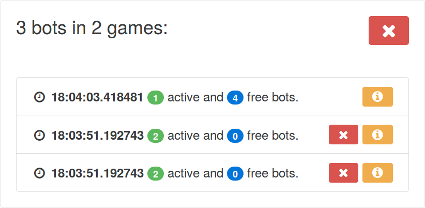
\includegraphics{assets/admin-games-list}
	\caption{Náhled seznamu her v administraci}
	\label{fig:admin-games-list}
\end{figure}

\begin{figure}[H]
	\centering
	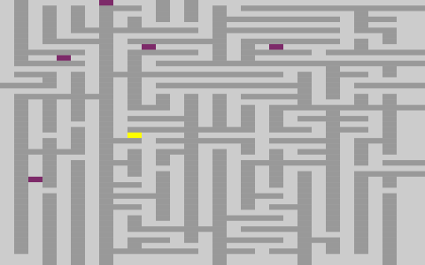
\includegraphics{assets/admin-game-detail}
	\caption{Náhled detailu hry v administraci}
	\label{fig:admin-game-detail}
\end{figure}

\begin{figure}[H]
	\centering
	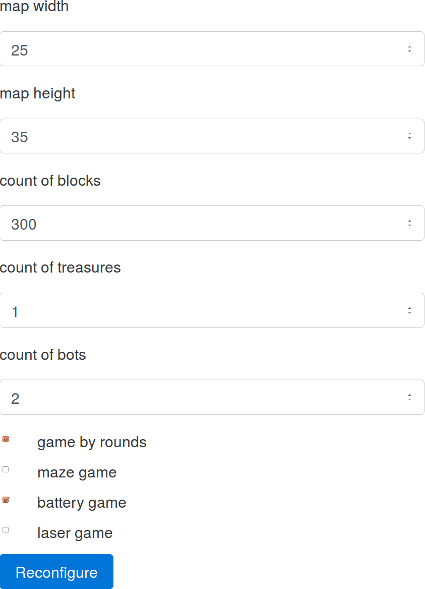
\includegraphics{assets/admin-conf-form}
	\caption{Náhled administračního formuláře pro konfiguraci}
	\label{fig:admin-conf-form}
\end{figure}
